\documentclass[a4paper,10pt]{article}

% ------------------------------------
% packages
\usepackage[a4paper,margin=1in,footnotesep=2.2\baselineskip]{geometry}
\usepackage{multicol}
\usepackage{xcolor}
\usepackage{framed}
\usepackage{emoji}
\usepackage[most]{tcolorbox}
\usepackage{fancyhdr}
\usepackage[tracking=true]{microtype}
\usepackage{ragged2e}
\usepackage{listings}
\usepackage{color}
\usepackage{pagecolor}
\usepackage{pdftexcmds}

% ------------------------------------
% checksum = SHA-1
\makeatletter
\ifx\pdf@filemdfivesum\undefined\def\pdf@filemdfivesum#{\mdfivesum file}\fi
\let\filesum\pdf@filemdfivesum
\makeatother

% ------------------------------------
% color definitions
\definecolor{armygreen}{rgb}{0.14, 0.71, 0.15}
\definecolor{darkgreen}{rgb}{0.08, 0.48, 0.18}
\definecolor{darkred}{rgb}{0.86, 0.153, 0.153}
\definecolor{azure}{rgb}{0.0, 0.5, 1.0}
\definecolor{bole}{rgb}{0.82, 0.57, 0.22}
\definecolor{dkgreen}{rgb}{0,0.6,0}
\definecolor{gray}{rgb}{0.5,0.5,0.5}
\definecolor{mauve}{rgb}{0.58,0,0.82}
\definecolor{light-gray}{gray}{0.95}
\definecolor{bg}{HTML}{fcfcfa}
\definecolor{bt}{HTML}{ffebe6}

% ------------------------------------
% code styling
\definecolor{shadecolor}{RGB}{180,180,180}
\newcommand{\code}[1]{\colorbox{shadecolor!30}{\mono{#1}}}
\colorlet{Gray}{gray!20!}
\tcbset{on line, arc=1pt, leftrule=0.25pt,rightrule=0.25pt,toprule=0.25pt,bottomrule=0.25pt,
	boxsep=3pt, left=0pt,right=0pt,top=0pt,bottom=0pt,
	colframe=white,colback=Gray,  
	highlight math style={enhanced}
}
\lstdefinelanguage{Solidity}{
  keywords={bool, true, false, return, address, bytes32, bytes4, bytes1, bytes, uint256, uint8, uint, string, if, while, else, case, break},
  keywordstyle=\color{blue}\bfseries,
  ndkeywords={function,struct, mapping, export, throw, implements, import, this},
  ndkeywordstyle=\color{darkgreen}\bfseries,
  identifierstyle=\color{black},
  sensitive=false,
  comment=[l]{//},
  morecomment=[s]{/*}{*/},
  commentstyle=\color{green}\mono,
  stringstyle=\color{orange}\mono,
  morestring=[b]',
  morestring=[b]",
  mathescape=true,
  literate={=>}{$\rightarrow{}$}{1}
}
\lstset{
  backgroundcolor=\color{light-gray},
  language=Solidity,
  aboveskip=3mm,
  belowskip=3mm,
  showstringspaces=false,
  columns=flexible,
  basicstyle={\small\mono},
  numbers=none,
  numberstyle=\tiny\color{gray},
  keywordstyle=\color{blue},
  commentstyle=\color{dkgreen},
  stringstyle=\color{mauve},
  breaklines=true,
  breakatwhitespace=true,
  tabsize=3
}

% ------------------------------------
% fonts
\newfontfamily\pro[Path=./]{SFMono.ttf}
\newfontfamily\pbold[Path=./]{SFMonoBold.ttf}
\newfontfamily\mono[Path=./]{SFMono.ttf}
\newfontfamily\mbold[Path=./]{SFMonoBold.ttf}

% ------------------------------------
% heading font-size
\usepackage{sectsty}
\usepackage{fontspec}
\sectionfont{\fontsize{12}{15}\selectfont}
\usepackage[utf8]{inputenc}

% ------------------------------------
% footnote positioning
\usepackage[hang,flushmargin,bottom]{footmisc} 

% ------------------------------------
% bibliography
\usepackage[colorlinks=true,
            linkcolor=blue,
            urlcolor=blue,
            citecolor=blue,
            pdfauthor={sshmatrix},
            pdftitle={Helix2 Protocol},
            pdfsubject={Link Service and Protocol},
            pdfkeywords={ethereum, account, abstraction, link, name, decentralised, distributed},
            pdfproducer={sshmatrix},
            pdfcreator={sshmatrix}]{hyperref}
            
% ------------------------------------
% blank footnote
\newcommand\blfootnote[1]{%
	\begingroup
	\renewcommand\thefootnote{}\footnote{#1}%
	\addtocounter{footnote}{-1}%
	\endgroup
}

% ------------------------------------
% header
\pagestyle{fancy}
\fancyhf{}
\lfoot{\footnotesize \mono{\#}\tcbox{\mono{\filesum{\jobname}}}}
\begin{document}
\setcounter{footnote}{0}
\newpage
\topskip15pt

\fancyhead[L]{\footnotesize \mono{author}:\tcbox{\mono{sshmatrix}}}
\fancyhead[R]{{\footnotesize \mono{\href{https://github.com/helix-coupler}{github.com/helix-coupler}}}}
\fancyhead[C]{{\footnotesize \emoji{dna}}}
\fancyfoot[C]{{\footnotesize \mono{\thepage/12}}}
\fancyfoot[R]{{\footnotesize \mono{\today} \emoji{dna}}}

\begin{center}
	\textbf{\Huge\pbold{HELIX2}}\\
	\vspace{0.075in}
	\textls[-50]{\mono{Link Service and Protocol}}\linebreak\linebreak
	\vspace{-0.175in}
	\textls[0]{\mono{sshmatrix}}\linebreak\linebreak
	\textls[0]{\mono{SysStruct}}\linebreak
	\textls[0]{\mono{\href{mailto:sshmatrix@pm.me}{sshmatrix@pm.me}}}\linebreak
\end{center}
\begin{center}
	\textbf{\Large\pbold{ABSTRACT}}\linebreak\linebreak
	\textls[-50]{\mono{Double Helix or Helix2 is a next-generation link service and account abstraction protocol on Ethereum, originally designed as a natural successor to generic name services. Helix2 protocol allows names to link to each other in several useful configurations on Ethereum blockchain. Helix2 infrastructure codifies interactions between names, categorises those interactions, assigns them rules and labels, and in some cases, validates those interactions with on-chain records. Due to its unique design crafted to leverage interactions among names, Helix2 enables names to form organised on-chain structures and graphs. Wallets integrating Helix2 can leverage its properties to provide users with a smart contract interface to transact and interact with the Ethereum blockchain; this arguably makes Helix2 an account abstraction infrastructure. }}
\end{center}
\vspace{0.2in}
\begin{flushleft}
	\textbf{\Large\pbold{INTRODUCTION}}\linebreak\linebreak
	\textls[-50]{\mono{Most blockchains have developed their own versions of naming systems which allow representing addresses with human-readable names. On Ethereum, \href{https://ens.domains}{Ethereum Name Service} (ENS) is the first and most notable example, while similar services later became available on Tezos and Solana in the form of \href{https://tezos.domains/en}{Tezos Domains} and \href{https://naming.bonfida.org/}{Solana Name Service} by Bonfida. By construction, a name service assigns names to nodes in a network. In a classic web2 world, Domain Name Service (DNS) fulfils this requirement. Crypto-native name services are similar to DNS in the sense that they enable assigning names to addresses similar to how DNS assigns human-readable names to Internet Protocols (IP). There are however clear added benefits to crypto-native naming architecture over DNS since crypto-native services often double as a decent identity framework in their respective blockchain ecosystems. It goes without saying that the immutability and decentralisation properties of typical crypto-native systems add to their desirability owing to their censor-resistant and unruggable nature.}}
\end{flushleft}
\begin{figure}[ht!]
 	\centering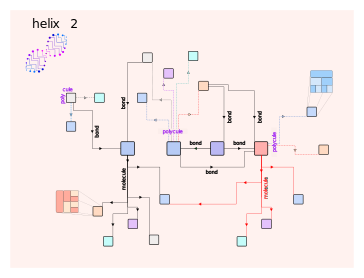
\includegraphics[width=160mm]{./schema/png/network.png}
	\mono{\caption{Helix2 Concept}}
	\label{fig:concept}
\end{figure}
\begin{flushleft}
	\textls[-50]{\mono{\href{https://helix2.xyz}{Helix2} is designed as a next-generation successor of these name services. While the set of nodes form a canonical and natural choice for labeling in any distributed system (e.g. addresses on any blockchain), the observation nonetheless is that most nodes do not interact with each other. For instance, there are about 220 million Ethereum addresses whereas an average address will likely interact with no more than a few hundred other addresses its lifetime. This means that most wallets have a limited set of interactions with contracts and addresses in general and their interactions are classifiable to a very large degree. Keeping this in mind, Helix2 is an attempt to provide Ethereum with a next-generation link service, in addition to the name service already provided by ENS. The expected outcome of the Helix2 protocol is a link-native naming ecosystem, a 'linkspace', where an interaction between two names is representable on-chain similar, but not limited to, a human-readable name for an address. A shift in focus from nodes to links has a profound effect on the nature of structures that an ecosystem can support. Several features which are challenging to achieve with a name service alone become extremely convenient with Helix2. For instance, Helix2 comes with several fundamental and easily accessible structural features such as stealth payments, social graphs, DAOs etc.\\
		\vspace{0.2in}
		While Helix2 has its own namespace, it does not replace ENS and is in fact intended to work alongside ENS as an extension. Helix2 is able to import all \tcbox{\mono{.}} namespaces by design without any bridging or wrapping. Lastly, Helix2 is not the only link service in the works; \href{https://woolball.xyz}{Woolball} is another link service currently under development although the two implementations arguably have more differences than similarities.\linebreak
	}}
\end{flushleft}
\begin{flushleft}
	\textbf{\large\pbold{DEFINITIONS}}\linebreak\linebreak
	\textls[-50]{\mono{
		Helix2 (Helix × 2) is roughly motivated by the double helix structure of DNA, where two polynucleotide chains are connected by bonds. The blockchain representation of this structure is two identical copies of the same blockchain connected by secure or unsecure bonds. The nomeclature is therefore borrowed from fundamental chemistry. Below is a list of definitions that will appear in this document:\linebreak\linebreak
		A {\mbold{name}} is an on-chain label for a node in a distributed system. An example of this is \tcbox{vitalik.eth} labeling the address of Vitalik on Ethereum.\linebreak\linebreak
		A {\mbold{link}} is an open relationship between two names where one name (source) may interact with another name (target) without latter's explicit approval. An example of a 'link' is  transfer of ERC20 or ERC721 tokens from one name to another, e.g. \tcbox{vitalik.eth} and \tcbox{virgil.eth} are linked via ERC interface.\linebreak\linebreak
		A source in Helix2 architecture is called a {\mbold{cation}}.\linebreak
		A target in Helix2 architecture is called an {\mbold{anion}}.\linebreak\linebreak
		A {\mbold{bond}} is a closed relationship between two names that requires explicit approval of both the cation (source) and the anion (target). An example of a bond is granting of controller permissions to an operator by an owner using ERC721 \tcbox{setApprovalForAll()} function. In this case, the interaction between the owner and controller is of closed nature\textsuperscript{\textcolor{blue}{1}}\blfootnote{\mono{\textsuperscript{1}Although this example uses addresses as nodes, a similar implementation is nonetheless possible with names.}}. In other words, a bond is a secure link since it requires explicit approval. Alternatively, a link is an unsecure bond.\linebreak\linebreak
		{\mbold{Covalence}} is a flag in Helix2 architecture that defines whether an interaction or relationship is a link or a bond. Covalence is \tcbox{true} for a secure bond and \tcbox{false} for an unsecure bond (aka link).\linebreak\linebreak
		A {\mbold{molecule}} is a set of similar bonds between a cation and several anions. An example of a molecule is the set of links between a DAO governor contract (source) and the participating token holders (targets). This molecule is secure since such membership of a DAO requires explicit approval of both the engaging entities. The individual bonds in this molecule are similar in the sense that the anions share the same relationship with the contract. A multi-sig vault is also an example of a molecule. A public channel in a Discord server is another example of a molecule.\linebreak\linebreak
		A {\mbold{polycule}} is a special type of molecule in which each individual bond between the cation and its several anions is unique. An example of a polycule is the set of private channels in a Discord server, where each channel may have its unique requirements as well as unique participating members.\linebreak\linebreak
		A {\mbold{hook}} is a contractual (or non-contractual) relationship (a contract) between two names. Technically, a hook is a map consisting of two elements \tcbox{rule $\rightarrow$ config}.\linebreak\linebreak
		A {\mbold{config}} is the address of the contract defining a hook between two names. For non-contractual relationships, \tcbox{0x0} config is used.\linebreak\linebreak
		A {\mbold{rule}} is an identifier which encodes the relationship between two names and must accompany a hook as its calldata.\linebreak\linebreak
	}}
\end{flushleft}
\begin{flushleft}
	\textbf{\Large\pbold{HELIX2 DESIGN}}\linebreak\linebreak\linebreak
	\textbf{\large\pbold{ETHEREUM NAME SERVICE (ENS)}}\linebreak\linebreak
	\textls[-50]{\mono{
		All name services so far have essentially been on-chain scalar databases (e.g. ENS, LENS, LNR, CB.ID), meaning that names are simply isolated nodes representable by one label (see figure textcolor{blue}{1} below). ENS is a good example of such a scalar architecture. Typical name services like ENS are also hierarchical namespaces in the sense that the set of subnodes and nodes form a merkle-tree with labels as leaves of the tree. In such an architecture, names are self-contained and isolated by construction. Refer to figure \textcolor{blue}{2}.
		}}\linebreak\linebreak\linebreak
	\textbf{\large\pbold{HELIX2 SERVICE}}\linebreak\linebreak
	\textls[-50]{\mono{
		Helix2 is essentially two services under one protocol: a native namespace providing a name service and a link service for that underlying namespace. Helix2 is an on-chain vector database. In Helix2, names can bond (or link) with one another; bonds are vectors between names, pointing from one name to another - this is the core premise of Helix2 protocol and essentially what separates it from other services. Helix2 names are not hierarchical, meaning that they cannot have subdomains, i.e. Helix2 is a flat namespace. Subdomains are not necessary in Helix2 since linking provides the same features without constraining the relationships between nodes to within one parent node's hierarchy. This is the only significant divergence of Helix2 namespace from ENS. In addition to this flat namespace, Helix2 has an additional linkspace which is the core utility of the protocol.
		\linebreak\linebreak
		While the theoretical premise of a linkspace appears easy, in practise, this premise requires some crucial modifications to work in a resource-constrained environment such as Ethereum Virtual Machine (EVM). One of these modifications consist of allowing one name to link with multiple names within one object with common or unique relationships among them. This is highly consequential in reducing gas costs for serial linkers.		
	}}
\end{flushleft}
\begin{figure}[ht!]
	\centering\includegraphics[width=160mm]{./schema/png/ens.png}
	\mono{\caption{Ethereum Name Service (ENS)}}
	\label{fig:ens}
\end{figure}
\begin{figure}[ht!]
	\centering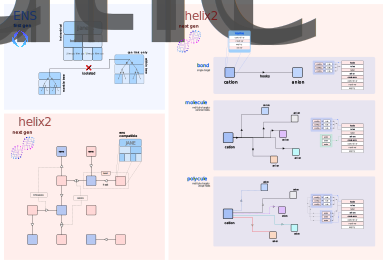
\includegraphics[width=160mm]{./schema/png/helix2.png}
	\mono{\caption{Helix2 Service}}
	\label{fig:helix2}
\end{figure}
\pagebreak
\begin{flushleft}
	\textbf{\Large\pbold{HELIX2 PROTOCOL}}\linebreak\linebreak
	\textls[-50]{\mono{
		All native objects (names, links, bonds etc) end with \tcbox{.}, e.g. \tcbox{alice.}, where \tcbox{.} acts as a trailing marker. Consequently, \tcbox{.} is one of the three reserved characters in Helix2 and cannot be used in any of the object labels (other than as a suffix).
		}}\linebreak\linebreak\linebreak
	\textbf{\large\pbold{NAMES}}
\end{flushleft}
\begin{lstlisting}

	struct NAME {
		address owner;
		address controller;
		address resolver;
		uint256 expiry;
	}
\end{lstlisting}
\begin{flushleft}
	\textls[-50]{\mono{
		Helix2 names are similar to ENS names, except that the suffix for them is\tcbox{.} instead of \tcbox{.eth}. Helix2 names are not hierarchical, meaning that they cannot have subdomains.\linebreak\linebreak
		All Helix2 names end with\tcbox{.} and they have a Resolver and Controller. Note again that\tcbox{.} is a reserved character and therefore forbidden. Additionally, \tcbox{\textcolor{purple}{-}} and\tcbox{\textcolor{blue}{\textcolor{blue}{\#}}} are also forbidden.
		}}\linebreak\linebreak
	\textbf{\normalsize\pbold{IMPORTING ENS NAMES}}\linebreak\linebreak
	\textls[-50]{\mono{
		Helix2 is capable of importing all \tcbox{.} namespaces by forbidding \tcbox{.} in its native namespace. In the prototype implementation of Helix2, ENS name import is already implemented and ENS users can claim their ENS on Helix2. For ENS names, the representation of names then looks like \tcbox{alice.eth.}, i.e. ENS name \tcbox{alice.eth} followed by a \tcbox{.} as the usual trailing marker.
		}}\linebreak\linebreak\linebreak
	\textbf{\large\pbold{BONDS}}
\end{flushleft}
\begin{lstlisting}

	struct BOND {
	    uint8[] rules;
	    mapping(uint8 => address) hooks;
	    bytes32 anion;
	    bytes32 label;
	    address resolver;
	    address controller;
	    bool covalence;
	    uint256 expiry;
	}
\end{lstlisting}
\begin{flushleft}
	\textls[-50]{\mono{
		A directional bond between two names \tcbox{alice.} $\rightarrow$ \tcbox{bob.} is labeled by its \tcbox{label}. Bonds start with \tcbox{\textcolor{blue}{-}}, end with \tcbox{.} and can be queried by their label prefixed with \tcbox{\textcolor{blue}{-}}, e.g. \tcbox{\textcolor{blue}{-}label.}.\linebreak\linebreak
		The source of the bond is called a cation (\tcbox{alice.}) and the target is called an anion (\tcbox{bob.}).
		}}\linebreak\linebreak
	\textls[-50]{\mono{
		Further, \tcbox{covalence} flag determines whether the bond is 'secure' or 'unsecure' (i.e. when the bond is in fact a link). To reiterate,\linebreak\linebreak
		\hspace*{0.2in}$\bullet$ a bond between alice and bob is insecure when it is uni-directional and requires only alice's approval, or a\linebreak\linebreak
		\hspace*{0.2in}$\bullet$ a bond between alice and bob is secure when it is mutual, bi-directional and requires both alice's and bob's approval.\linebreak\linebreak
		Covalence can be set (\tcbox{true}) or unset (\tcbox{false}) through co-signing a message (2/2 multi-sig) by the cation and the anion.
		}}\linebreak\linebreak\linebreak
	\textbf{\large\pbold{HOOKS, RULES \& CONFIG}}\linebreak\linebreak
	\textls[-50]{\mono{
		The most important features of bonds are \tcbox{config} and \tcbox{rules}, combining to form \tcbox{hooks}, which quantify the link between two names and give meaning to the \tcbox{\textcolor{blue}{-}} representation. Hooks are contractual mappings \tcbox{rule $\rightarrow$ config} between two names mediated by ordered one-to-one mapping inside \tcbox{\textcolor{blue}{uint8}[] rules}: \tcbox{\textcolor{darkgreen}{mapping}(\textcolor{blue}{uint8} $\rightarrow$ \textcolor{blue}{address}) hooks;}\linebreak\linebreak
		\hspace*{0.2in}$\bullet$ To query a hook's config inside \tcbox{hooks} for a bond, one needs its associated \tcbox{rule}, which is a \tcbox{uint8} identifier mapping to the contractual address \tcbox{config}. Hooks are thus queryable as \tcbox{\textcolor{blue}{-}label\textcolor{blue}{\textcolor{blue}{\#}}rule.}, e.g. \tcbox{\textcolor{blue}{-}label\textcolor{blue}{\textcolor{blue}{\#}}404.}.\linebreak\linebreak
		\hspace*{0.2in}$\bullet$ A trivial application of a hook is a payment router, i.e. payment sent to \tcbox{0} hook \tcbox{\textcolor{blue}{-}label\textcolor{blue}{\textcolor{blue}{\#}}0.} is routed to the address of \tcbox{bob.}; more on hooks in upcoming sections.\linebreak
		}}\linebreak\linebreak
	\textbf{\large\pbold{MOLECULES}}
\end{flushleft}
\begin{lstlisting}

	struct MOLECULE {
	    uint8[] rules;
	    mapping(uint8 => address) hooks;
	    bytes32[] anions;
	    bytes32 label;
	    address resolver;
	    address controller;
	    bool covalence;
	    uint256 expiry;
	}
\end{lstlisting}
\begin{flushleft}
	\textls[-50]{\mono{
		Helix2 allows for multi-bonding such that a cation can bond with multiple anions within one data structure instead of creating individual (and costlier) bonds; this structure is called a 'molecule' (or 'moly' in short). In a molecule, all individual bonds share the same covalence.\linebreak\linebreak
		Other features of a molecule are similar to that of a bond, e.g. a molecule can have an label and hooks. To denote a bond with label \tcbox{label}, we use two consecutive \tcbox{\textcolor{blue}{-\,-}} characters, i.e. \tcbox{\textcolor{blue}{-\,-}label.} without refering to an anion since molecules are anion-agnostic and hook-independent. By using \tcbox{\textcolor{blue}{-\,-}label\textcolor{blue}{\textcolor{blue}{\#}}rule.}, one can refer to a unique hook for a molecule. Covalence can be set (\tcbox{true}) or unset (\tcbox{false}) through co-signing a message by the cation and all the anions.
		}}\linebreak\linebreak\linebreak
	\textbf{\large\pbold{POLYCULES}}
\end{flushleft}
\lstset{emph={rules,hooks,anions}, emphstyle=\textcolor{purple}}
\begin{lstlisting}

	struct POLYCULE {
	    uint8[] rules;
	    mapping(uint8 => address) hooks;
	    bytes32[] anions;
	    bytes32 label;
	    address resolver;
	    address controller;
	    bool covalence;
	    uint256 expiry;
	}
\end{lstlisting}
\begin{flushleft}
	\textls[-50]{\mono{
		Lastly, we can define another useful abstraction in the form of a 'polycule', which is a molecule comprising of unique bonds between a cation and a set of anions. In a polycule, all individual bonds share the same covalence despite being unique. In short, \tcbox{rules\textcolor{blue}{.length} == anions\textcolor{blue}{.length}}, and \tcbox{rules} \& \tcbox{anions} are a one-to-one map.\linebreak\linebreak
		Other features of a molecule are similar to that of a molecule. To denote a bond with label \tcbox{label}, we use three consecutive \tcbox{\textcolor{blue}{-\,-\,-}} characters, i.e. \tcbox{\textcolor{blue}{-\,-\,-}label.}  etc. By using \tcbox{\textcolor{blue}{-\,-\,-}label\textcolor{blue}{\#}rule.}, one can refer to a unique hook for a molecule by its \tcbox{rule}. Alternatively, one can refer to a unique anion in a molecule by its indexed \tcbox{rule}, e.g. \tcbox{\textcolor{blue}{-\,-\,-}label\textcolor{blue}{\#}anions[rule]}. Covalence can be set or unset through co-signing a message by the cation and all the anions.
	}}
\end{flushleft}
\begin{figure}[ht!]
	\centering\includegraphics[width=160mm]{./schema/png/struct.png}
	\mono{\caption{Helix2 Classes}}
	\label{fig:classes}
\end{figure}
\begin{flushleft}
	\textls[-50]{\mono{
		The \tcbox{molecule} structure is a topological superset i.e. it is possible to derive polycules and bonds from molecules although that'll literally be a gas-guzzling mistake. The seemingly unnecessary differentiation between the three is to optimise gas consumption. Helix2 architecture leaves room for future upgrades with new submodules. These submodules may be referenced by their integer index N as \tcbox{\textcolor{blue}{-\,N\,-}label\textcolor{blue}{\#}rule.}, e.g \tcbox{\textcolor{blue}{-\,42\,-}vitalink\textcolor{blue}{\#}404.}.
		}}\linebreak\linebreak\linebreak
	\textbf{\Large\pbold{CONTRACTS}}\linebreak\linebreak
	\textls[-50]{\mono{
		Helix2 Protocol is a fairly large set of code divided into clean modules in a way that all submodules are replaceable and upgradeable without breaking any existing architecture or interfaces. This is achieved through a combination of basic logic \& storage separation via proxies and \href{https://eips.ethereum.org/EIPS/eip-2535}{EIP-2535 Diamond Standard}.\linebreak\linebreak
	}}
\end{flushleft}
\begin{figure}[ht!]
	\centering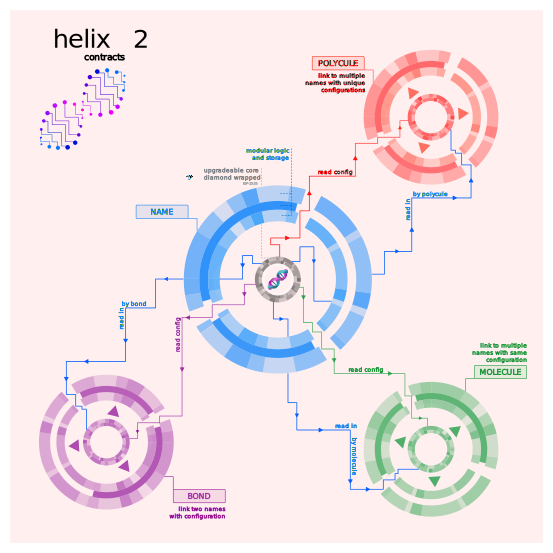
\includegraphics[width=160mm]{./schema/png/contracts.png}
	\mono{\caption{Helix2 Contracts}}
	\label{fig:contracts}
\end{figure}
\begin{flushleft}
	\textls[-50]{\mono{
		There are four submodules in the genesis version of protocol - Name, Bond, Molecule and Polycule. Each submodule is composed of three contracts - Registrar, Registry \& Storage. In each submodule, the storage contracts are proxied by registry contracts such that the logic and storage is seperated. This enables the protocol to replace the storage and logic in each submodule seemlessly through future protocol upgrades without compromising on-top services. Name submodule is somewhat more central to the architecture than the remaining three link modules since links depend on and derive from names.\linebreak\linebreak
		The four submodules are connected at the core by the Helix2 Core manager which is the bespoke state-of-the-art Multi-facet Proxy (EIP-2535). EIP-2535 compliant contracts are fully upgradeable and it allows Helix2 protocol to use one single address forever without compromising on future functionalities or breaking existing on-chain or off-chain functionalities. Helix2 manager is capable of excepting new submodules, replace existing submodules or update core configuration.\linebreak\linebreak\linebreak
		}}
	\textbf{\Large\pbold{ACCOUNT ABSTRACTION}}\linebreak\linebreak
	\textls[-50]{\mono{
		Helix2 is a core infrastructure which can be leveraged for perhaps countless utilities. One of the biggest utilities of Helix2 arises in account abstraction. {\pbold A}ccount {\pbold A}bstraction (AA) is an umbrella term first defined in \href{https://eips.ethereum.org/EIPS/eip-2938}{EIP-2938}, to categorise infrastructures that allow the use of smart contracts as wallets instead of the typical logic-free 'externally owned accounts' (EOA) that are currently in use as wallets. The core ideology behind account abstraction is to allow users to arbitrarily customise their handling of transactions, funds and interactions with the Ethereum blockchain in general with smart contract code.\linebreak
		
		Several decentralised applications (dApps) on Ethereum already allow specific smart control over blockchain interactions (e.g. \href{https://safe.global/}{Gnosis Vault}, \href{https://app.umbra.cash}{Umbra Cash}, \href{https://tornadocash.eth.link/}{Tornado Cash}, \href{https://opengsn.org/}{Gas Station Network}) but this list is rather small and the utility of them rather limited to only a few aspects. These services may additionally require users to pay additional fees on top of the (un)optimised gas costs. \linebreak
		
		EIP-2938 proposed a new set of \tcbox{OPCODES} that would allow account abstraction at core level but this required significant non-trivial changes to Ethereum consensus layer. \href{https://eips.ethereum.org/EIPS/eip-4337}{EIP-4337} proposed another infrastructure that uses alternative mempools ('alt mempools') for bundling transactions and then routing them to the consensus layer upon validation (akin to \href{https://www.flashbots.net/}{Flashbots}); the alt mempools would then be responsible for validating the smart wallet transaction calls and thereby such a validation \& routing environment remains independent of the primary mempool and wouldn't require changes to the consensus layer itself. Due to the independent nature of the alt mempools, there is also room for mempool-level optimisations (e.g. of bundlers) to further minimise gas costs which is usually not the case for typical dApps.\linebreak
		
		Helix2 is also an account abstraction infrastructure that uses a namespace and its associated linkspaces, i.e. data structures containining pointers to smart contracts from names, to act as a router of transactions for any name (see figure \textcolor{blue}{6}). Since the name- and linkspace are disjoint from the underlying EOA, the user pays no other gas costs than the standard network transaction fees, excluding the one-time cost of writing the pointers in the Helix2 data structure. Wallets connecting users to the blockchain via their names are therefore abstracted by Helix2 since the user can insert arbitrary logic to their name- and linkspace. ENS already provides a fraction of this functionality but loses out on the ability to enforce dynamic arbitrary front-facing logic due to its heirarchical nature. The several specific usecases of Helix2 mentioned in the upcoming sections are all examples of account abstraction.
	}}
\end{flushleft}
\begin{figure}[ht!]
 	\centering\includegraphics[width=160mm]{./schema/png/abstraction.png}
	\mono{\caption{Account Abstraction built on Helix2}}
	\label{fig:aa}
\end{figure}
\begin{flushleft}
	\textbf{\large\pbold{MULTI-SIG VAULTS}}\linebreak\linebreak
	\textls[-50]{\mono{
		By design, Helix2 molecules are a perfect fit for multi-sig vault management. Molecule struct is readily mappable to a multi-sig safe architecture and it readily formalises vaults as nameable linkspaces. In fact, Helix2 can store multiple vault agreements among a set of parties inside a single standard struct.\linebreak\linebreak
	}}
	\textbf{\large\pbold{STEALTH PAYMENTS}}\linebreak\linebreak
	\textls[-50]{\mono{
		Helix2 hooks can be configured for bonds to receive stealth payments to a name via a stealth protocol such as \href{https://github.com/ScopeLift/umbra-protocol}{Umbra Protocol} or \href{https://zk.money/}{Aztec}. Note that this feature is also possible with ENS Resolver. In addition however, Helix2 allows performing stealth payments enmasse and with better control over sensitive data streams.\linebreak\linebreak
	}}
	\textbf{\large\pbold{WEB3 SOCIAL GRAPHS}}\linebreak\linebreak
	\textls[-50]{\mono{
		Helix2 molecules are a natural fit for open social graphs and could aid in better decentralised social media protocols. In the current implementation, molecules are an appropriate representation of social groupings, although a complete version requires one or more submodules that can link molecules and polycules among each other. This requirement may vary from one platform to another, and is therefore not part of the Helix2 core protocol.\linebreak\linebreak
	}}
	\textbf{\large\pbold{MESSAGING \& CHAT APPS}}\linebreak\linebreak
	\textls[-50]{\mono{
		Helix2 molecules are a natural fit for web3 messaging apps and chat services. In particular, molecules are a canonical choice for organising group chat participants and their permissions whereas polycules could be utilised to manage private channels. Both in combination could help build the elusive web3 version of Discord.\linebreak\linebreak
	}}
	\textbf{\large\pbold{DAO}}\linebreak\linebreak
	\textls[-50]{\mono{
		Helix2 molecules are a canonical fit for DAO governance and associated tooling where delegates can be viewed as members of the same molecule with common relationship among all members of the DAO. \href{https://orca.mirror.xyz/Y2xvPmB4cJH51srGqY6Mm_g38lV-7cwvtyDePnyzfAE}{Orca Protocol} is a similar idea which has been implemented already albeit with limited focus on on-chain coordination. Helix2 in comparison makes the same task significantly easier at protocol level and allows formation of highly complex pods at much lower architectural cost.\linebreak\linebreak
	}}
	\textls[-50]{\mono{
		Helix2 molecules are a canonical fit for DAO governance and associated tooling where delegates can be viewed as members of the same molecule with common relationship among all members of the DAO. \href{https://orca.mirror.xyz/Y2xvPmB4cJH51srGqY6Mm_g38lV-7cwvtyDePnyzfAE}{Orca Protocol} is a similar idea which has been implemented already albeit with limited focus on on-chain coordination. Helix2 in comparison makes the same task significantly easier at protocol level and allows formation of highly complex pods at much lower architectural cost.\linebreak\linebreak
	}}
	\textbf{\large\pbold{OTHER UTILITIES}}\linebreak\linebreak
	\textls[-50]{\mono{
		Other possible use-cases include\linebreak\linebreak
		\hspace*{0.2in}$\bullet$ a unified web3 individual and group reputation system,\linebreak\linebreak
		\hspace*{0.2in}$\bullet$ proof-of-humanness by defining human-specific hooks in molecules or polycules,\linebreak\linebreak
		\hspace*{0.2in}$\bullet$ and perhaps anything and everything that requires structuring in groups.\linebreak\linebreak\linebreak
		}}
		\textbf{\Large\pbold{FUTURE}}\linebreak\linebreak
		\textls[-50]{\mono{The architecture of Helix2 service described in this paper promises several advances and features with clear utility across the Ethereum ecosystem ranging from identity to stealth payments.
		}}
\end{flushleft}
\begin{figure}[h]
	\centering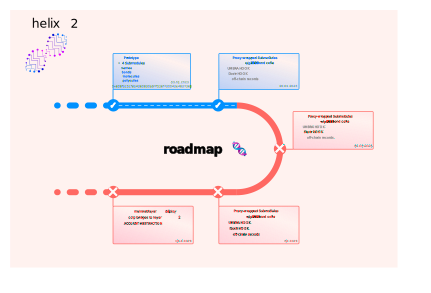
\includegraphics[width=160mm]{./schema/png/roadmap.png}
	\mono{\caption{Helix2 Roadmap}}
	\label{fig:roadmap}
\end{figure}
\begin{flushleft}
	\textls[-50]{\mono{Nonetheless, it will be naive to think that its usecases will be limited to what is discussed in this paper. The architecture of Helix2 protocol is fairly low level and it has been designed for maximum upgradeability and dynamism with as little friction as possible. The four submodules introduced in this paper are only the most basic structures and the Helix2 core expects several new submodules in the future under its repertoire.\linebreak\linebreak
	The codebase of Helix2 at the time of writing is at a fairly advanced stage with its upgradeable core and the initial set of four submodules in place (see figure \textcolor{blue}{6}). In near future, Helix2 expects to integrate off-chain lookups for extremely large link structures using \href{https://chain.link/cross-chain}{Chainlink's CCIP Protocol}, integrate presets for stealth payments (via \href{https://github.com/ScopeLift/umbra-protocol}{Umbra}) and a bridge to \href{https://dostr-eth.github.io/homepage/}{Dostr} - an Ethereum-flavoured \href{https://nostr.com/}{Nostr} client. Upon completion of these tasks, full Helix2 Protocol will be deployed on Ethereum Mainnet L1, with CCIP bridges to all primary L2 chains such as Optimism, zkSync, Starknet etc following soon after. Coordinates of the WIP codebase are at the end of the document.\linebreak\linebreak\linebreak
	}}
	\textbf{\large\pbold{ACKNOWLEDGEMENTS}}\linebreak\linebreak
	\textls[-50]{\mono{Helix2 is a work in progress and we thank \tcbox{0xc0de4c0ffee} for their valuable insights. We invite individuals and parties with interest in contributing to Helix2 protocol to get in touch via Github. 
	}}\linebreak\linebreak\linebreak
\end{flushleft}
\pagebreak
\begin{flushleft}
	\textbf{\Large\pbold{REFERENCES}}\linebreak\linebreak
		\textls[-50]{\mono{
			Ethereum Name Service (ENS): \href{https://ens.domains}{ens.domains}\linebreak
			Tezos Domains: \href{https://tezos.domains/en}{tezos.domains}\linebreak
			Solana Name Service: \href{https://naming.bonfida.org/}{naming.bonfida.org}\linebreak
			Woolball: \href{https://woolball.xyz}{woolball.xyz}\linebreak
			EIP-2535 Diamond Standard: \href{https://eips.ethereum.org/EIPS/eip-2535}{EIP-2535}\linebreak
			Umbra Protocol: \href{https://app.umbra.cash/}{umbra.cash}\linebreak
			Aztec Protocol: \href{https://zk.money/}{zk.money}\linebreak
			Orca Protocol: \href{https://orca.mirror.xyz/Y2xvPmB4cJH51srGqY6Mm_g38lV-7cwvtyDePnyzfAE}{orca.mirror}\linebreak
			Cross-Chain Interoperability Protocol (CCIP): \href{https://chain.link/cross-chain}{chain.link/cross-chain}\linebreak
			Aztec Protocol: \href{https://zk.money/}{zk.money}\linebreak
			Nostr ({\pbold{N}}otes and {\pbold{O}}ther {\pbold{S}}tuff {\pbold{T}}ransmitted by {\pbold{R}}elays): \href{https://nostr.com}{nostr.com}\linebreak
			Dostr (Ethereum-flavoured Nostr): \href{https://dostr-eth.github.io/homepage/}{dostr-eth}\linebreak
			EIP-2938 (Account Abstraction): \href{https://eips.ethereum.org/EIPS/eip-2938}{EIP-2938}\linebreak
			EIP-4337 (Account Abstraction Using Alt Mempool): \href{https://eips.ethereum.org/EIPS/eip-4337}{ERC-4337}\linebreak
			Maximum Extractable Value (MEV) \& Flashbots: \href{https://www.flashbots.net/}{Flashbots}\linebreak
			Tornado Cash dApp: \href{https://tornadocash.eth.link/}{Tornado.Cash}\linebreak
			Gas Station Network dApp: \href{https://opengsn.org/}{OpenGSN.org}\linebreak
			\linebreak\linebreak
		}}
\end{flushleft}
\begin{flushright}
	\textbf{\large\pbold{METADATA}}\linebreak\linebreak
	\textls[-50]{\mono{
		\mono{Github: }\tcbox{\mono{\href{https://github.com/helix-coupler}{github.com/helix-coupler}}}\linebreak
		\mono{Contracts: }\tcbox{\mono{\href{https://github.com/helix-coupler}{github.com/helix-coupler/helix2-contracts}}}\linebreak
		\mono{Source: }\tcbox{\mono{\href{https://github.com/helix-coupler}{github.com/helix-coupler/resources}}}\linebreak
		\mono{SHA-1 Checksum: }\tcbox{\mono{\href{https://github.com/helix-coupler/resources/blob/master/yellow-paper/helix2.tex}{\filesum{\jobname}}}}\linebreak
		\mono{Date: }\tcbox{\mono{\today}}\linebreak
	}}
\end{flushright}
\end{document}
